\chapter{The Geometry of Conceptualisation: Analogies} \label{chap:analogy}

\section{Analogies as Parallel Vectors}

\begin{figure}
%  \centering
  \begin{subfigure} [t] {0.5\textwidth}
  \centering
  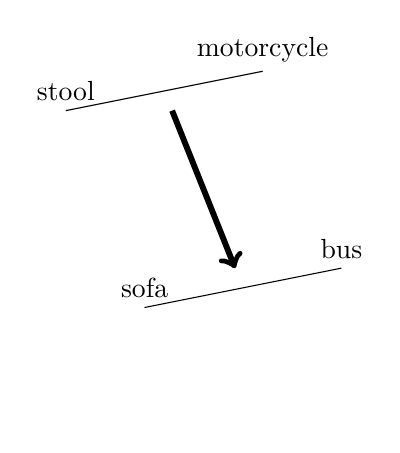
\begin{tikzpicture} [scale = 0.05]
    \draw (10,80)--(60,90);
    \draw (10,80) [above] node {stool};
    \draw (60,90) [above] node{motorcycle};
    \draw (30,30)--(80,40);
    \draw (30,30) [above] node {sofa};
    \draw (80,40) [above] node {bus};
    \draw [->,line width = 0.75 mm] (37,80)--(53,40);
    \draw (60,10) [below,white] node {soft};
  \end{tikzpicture}
  \caption{This makes sense.}
  \end{subfigure}
  \begin{subfigure} [t] {0.5\textwidth}
  \centering
  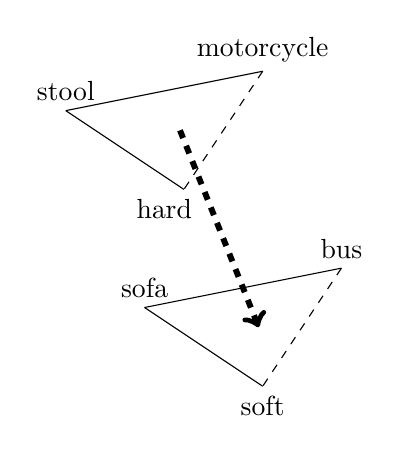
\begin{tikzpicture} [scale = 0.05]
    \draw (10,80)--(60,90);
    \draw (10,80)--(40,60);
    \draw [dashed] (60,90)--(40,60);
    \draw (10,80) [above] node {stool};
    \draw (60,90) [above] node {motorcycle};
    \draw (35,60) [below] node {hard};
    \draw (30,30)--(80,40);
    \draw (30,30)--(60,10);
    \draw [dashed] (80,40)--(60,10);
    \draw (30,30) [above] node {sofa};
    \draw (80,40) [above] node {bus};
    \draw (60,10) [below] node {soft};
    \draw [->,line width = 0.75 mm,dashed] (39,75)--(59,25);
  \end{tikzpicture}
  \caption{Does this make sense?}
  \end{subfigure}
\caption[Analogies Straining Geometry]{The analogical components of overlapping conceptual frames do not necessarily map neatly into a singular space.}
\end{figure}

\section{Contextualising Analogical Geometry}

\begin{figure}
\centering
\begin{subfigure} [t] {0.3 \textwidth}
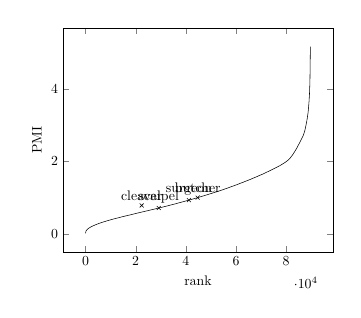
\begin{tikzpicture}[scale=0.5]
	\begin{axis} [xlabel=rank,ylabel=PMI]
	\addplot [mark=none] coordinates {
		(0,0.00622) (179,0.06993) (358,0.08958) (537,0.1038) (716,0.11612) (895,0.1277) (1074,0.13863) (1253,0.14843) (1432,0.15739) (1611,0.16389) (1790,0.17189) (1969,0.17942) (2148,0.18635) (2327,0.19268) (2506,0.19919) (2685,0.20512) (2864,0.21109) (3043,0.21663) (3222,0.22214) (3401,0.22756) (3580,0.23298) (3759,0.23843) (3938,0.24394) (4117,0.24876) (4296,0.25433) (4475,0.25886) (4654,0.26335) (4833,0.26848) (5012,0.27326) (5191,0.2776) (5370,0.28219) (5549,0.28689) (5728,0.29159) (5907,0.29576) (6086,0.29963) (6265,0.30341) (6444,0.30759) (6623,0.31191) (6802,0.31573) (6981,0.31984) (7160,0.32383) (7339,0.32767) (7518,0.33159) (7697,0.33524) (7876,0.33996) (8055,0.34371) (8234,0.34751) (8413,0.35149) (8592,0.35495) (8771,0.3588) (8950,0.36238) (9129,0.36589) (9308,0.3694) (9487,0.37303) (9666,0.37628) (9845,0.37978) (10024,0.38348) (10203,0.38663) (10382,0.39019) (10561,0.39335) (10740,0.39672) (10919,0.39989) (11098,0.40352) (11277,0.40669) (11456,0.40985) (11635,0.41317) (11814,0.41601) (11993,0.41905) (12172,0.42228) (12351,0.42574) (12530,0.42889) (12709,0.43215) (12888,0.43526) (13067,0.43861) (13246,0.44192) (13425,0.44501) (13604,0.44801) (13783,0.45097) (13962,0.45451) (14141,0.45782) (14320,0.46114) (14499,0.4642) (14678,0.46746) (14857,0.47018) (15036,0.47349) (15215,0.47674) (15394,0.47975) (15573,0.4826) (15752,0.48588) (15931,0.4887) (16110,0.49164) (16289,0.49459) (16468,0.49724) (16647,0.50011) (16826,0.50297) (17005,0.50606) (17184,0.50888) (17363,0.51207) (17542,0.51475) (17721,0.51782) (17900,0.5208) (18079,0.52378) (18258,0.52714) (18437,0.53026) (18616,0.5329) (18795,0.53599) (18974,0.53886) (19153,0.54177) (19332,0.54494) (19511,0.548) (19690,0.55123) (19869,0.55423) (20048,0.55704) (20227,0.56012) (20406,0.56341) (20585,0.56611) (20764,0.56916) (20943,0.57217) (21122,0.57508) (21301,0.57829) (21480,0.58135) (21659,0.58423) (21838,0.58723) (22017,0.59032) (22196,0.59322) (22375,0.59608) (22554,0.59926) (22733,0.60207) (22912,0.60469) (23091,0.60727) (23270,0.61001) (23449,0.61277) (23628,0.61591) (23807,0.61897) (23986,0.62215) (24165,0.6252) (24344,0.6282) (24523,0.63076) (24702,0.63338) (24881,0.63622) (25060,0.63937) (25239,0.64226) (25418,0.64501) (25597,0.64812) (25776,0.65131) (25955,0.65425) (26134,0.65743) (26313,0.66062) (26492,0.66364) (26671,0.66654) (26850,0.66942) (27029,0.67227) (27208,0.67511) (27387,0.67796) (27566,0.68096) (27745,0.68396) (27924,0.68686) (28103,0.6899) (28282,0.69294) (28461,0.69609) (28640,0.69923) (28819,0.70204) (28998,0.70543) (29177,0.70847) (29356,0.71139) (29535,0.71433) (29714,0.71735) (29893,0.71996) (30072,0.72312) (30251,0.72642) (30430,0.72947) (30609,0.7324) (30788,0.73545) (30967,0.73833) (31146,0.74182) (31325,0.74495) (31504,0.74811) (31683,0.75129) (31862,0.75405) (32041,0.75737) (32220,0.76061) (32399,0.76356) (32578,0.7666) (32757,0.76932) (32936,0.77241) (33115,0.77588) (33294,0.77932) (33473,0.78278) (33652,0.78562) (33831,0.78914) (34010,0.79218) (34189,0.79538) (34368,0.79877) (34547,0.80197) (34726,0.8054) (34905,0.80829) (35084,0.81143) (35263,0.81449) (35442,0.81771) (35621,0.82091) (35800,0.82416) (35979,0.8272) (36158,0.83062) (36337,0.83407) (36516,0.83756) (36695,0.84107) (36874,0.84487) (37053,0.84793) (37232,0.85153) (37411,0.85447) (37590,0.85752) (37769,0.86058) (37948,0.86373) (38127,0.86726) (38306,0.87084) (38485,0.87456) (38664,0.87753) (38843,0.88126) (39022,0.8846) (39201,0.88825) (39380,0.89193) (39559,0.89522) (39738,0.89852) (39917,0.90171) (40096,0.90478) (40275,0.90875) (40454,0.91248) (40633,0.91579) (40812,0.91892) (40991,0.92276) (41170,0.92593) (41349,0.92932) (41528,0.93243) (41707,0.93626) (41886,0.93965) (42065,0.94308) (42244,0.94683) (42423,0.95023) (42602,0.95332) (42781,0.95676) (42960,0.96013) (43139,0.96401) (43318,0.96757) (43497,0.97095) (43676,0.97457) (43855,0.97845) (44034,0.98163) (44213,0.98517) (44392,0.98905) (44571,0.99275) (44750,0.99655) (44929,1.0005) (45108,1.00397) (45287,1.00741) (45466,1.01108) (45645,1.01478) (45824,1.01889) (46003,1.02265) (46182,1.02606) (46361,1.02949) (46540,1.03321) (46719,1.0376) (46898,1.04151) (47077,1.04542) (47256,1.04862) (47435,1.05241) (47614,1.0561) (47793,1.06009) (47972,1.06438) (48151,1.06797) (48330,1.07158) (48509,1.07559) (48688,1.07923) (48867,1.08319) (49046,1.08722) (49225,1.09178) (49404,1.09569) (49583,1.09919) (49762,1.10272) (49941,1.10649) (50120,1.11012) (50299,1.11343) (50478,1.11751) (50657,1.12162) (50836,1.12529) (51015,1.129) (51194,1.13319) (51373,1.13788) (51552,1.14134) (51731,1.14586) (51910,1.14935) (52089,1.15353) (52268,1.15734) (52447,1.16138) (52626,1.1649) (52805,1.16941) (52984,1.17299) (53163,1.17754) (53342,1.18187) (53521,1.18572) (53700,1.18992) (53879,1.19402) (54058,1.19822) (54237,1.2028) (54416,1.20724) (54595,1.21153) (54774,1.21532) (54953,1.21968) (55132,1.22365) (55311,1.22821) (55490,1.23284) (55669,1.23688) (55848,1.24146) (56027,1.24596) (56206,1.25055) (56385,1.25462) (56564,1.25882) (56743,1.26278) (56922,1.26691) (57101,1.27167) (57280,1.27617) (57459,1.28033) (57638,1.28496) (57817,1.29007) (57996,1.29527) (58175,1.29949) (58354,1.30419) (58533,1.30862) (58712,1.31248) (58891,1.31693) (59070,1.32147) (59249,1.326) (59428,1.33084) (59607,1.33539) (59786,1.33987) (59965,1.34406) (60144,1.34878) (60323,1.35337) (60502,1.35816) (60681,1.36334) (60860,1.36826) (61039,1.37278) (61218,1.37756) (61397,1.38269) (61576,1.38757) (61755,1.39261) (61934,1.39714) (62113,1.40166) (62292,1.40597) (62471,1.41042) (62650,1.41491) (62829,1.41951) (63008,1.42551) (63187,1.4301) (63366,1.43542) (63545,1.43978) (63724,1.44486) (63903,1.45018) (64082,1.45489) (64261,1.45996) (64440,1.46479) (64619,1.46885) (64798,1.47403) (64977,1.4791) (65156,1.484) (65335,1.48895) (65514,1.49372) (65693,1.49862) (65872,1.50393) (66051,1.50995) (66230,1.51516) (66409,1.5204) (66588,1.52569) (66767,1.53057) (66946,1.5358) (67125,1.54088) (67304,1.54632) (67483,1.5512) (67662,1.55641) (67841,1.56197) (68020,1.56758) (68199,1.5728) (68378,1.57798) (68557,1.58299) (68736,1.58852) (68915,1.59337) (69094,1.59947) (69273,1.60513) (69452,1.61009) (69631,1.61542) (69810,1.62112) (69989,1.62618) (70168,1.63211) (70347,1.63643) (70526,1.6416) (70705,1.64784) (70884,1.65311) (71063,1.65867) (71242,1.66373) (71421,1.67018) (71600,1.67668) (71779,1.68261) (71958,1.68941) (72137,1.69485) (72316,1.70138) (72495,1.70665) (72674,1.71271) (72853,1.71846) (73032,1.72475) (73211,1.73033) (73390,1.73666) (73569,1.74316) (73748,1.74971) (73927,1.75572) (74106,1.76177) (74285,1.76787) (74464,1.77402) (74643,1.78022) (74822,1.78605) (75001,1.7915) (75180,1.79783) (75359,1.80407) (75538,1.80936) (75717,1.81584) (75896,1.82204) (76075,1.82837) (76254,1.83537) (76433,1.84117) (76612,1.84712) (76791,1.85413) (76970,1.86132) (77149,1.86823) (77328,1.8738) (77507,1.88035) (77686,1.88647) (77865,1.89359) (78044,1.90222) (78223,1.90897) (78402,1.91791) (78581,1.92419) (78760,1.93224) (78939,1.9403) (79118,1.94828) (79297,1.95543) (79476,1.96368) (79655,1.97165) (79834,1.98096) (80013,1.99021) (80192,1.99859) (80371,2.00809) (80550,2.01824) (80729,2.02866) (80908,2.0393) (81087,2.05115) (81266,2.06415) (81445,2.07645) (81624,2.09072) (81803,2.10798) (81982,2.12461) (82161,2.13872) (82340,2.15538) (82519,2.17155) (82698,2.19041) (82877,2.20763) (83056,2.22721) (83235,2.2473) (83414,2.26669) (83593,2.28871) (83772,2.30865) (83951,2.32968) (84130,2.35005) (84309,2.37126) (84488,2.39428) (84667,2.41776) (84846,2.44125) (85025,2.46588) (85204,2.48839) (85383,2.51048) (85562,2.5345) (85741,2.55836) (85920,2.5831) (86099,2.61013) (86278,2.63505) (86457,2.66057) (86636,2.68674) (86815,2.713) (86994,2.74309) (87173,2.78014) (87352,2.81878) (87531,2.86846) (87710,2.92534) (87889,2.98645) (88068,3.04816) (88247,3.11264) (88426,3.18631) (88605,3.2714) (88784,3.35855) (88963,3.50245) (89142,3.65465) (89321,3.85875) (89500,4.20406) (89679,5.16929)
	};
	\addplot [mark=x,only marks] coordinates {
		(29204,0.70908)(22377,0.77903)(41247,0.92747)(44737,0.99632)
	};
	\node [anchor=south] at (axis cs: 29204,0.70908) {scalpel};
	\node [anchor=south] at (axis cs: 22377,0.77903) {cleaver};
	\node [anchor=south] at (axis cs: 41247,0.92747) {surgeon};
	\node [anchor=south] at (axis cs: 44737,0.99632) {butcher};
	\end{axis}
\end{tikzpicture}
\caption{dimension: \emph{life}}
\end{subfigure}
\centering
\begin{subfigure} [t] {0.3 \textwidth}
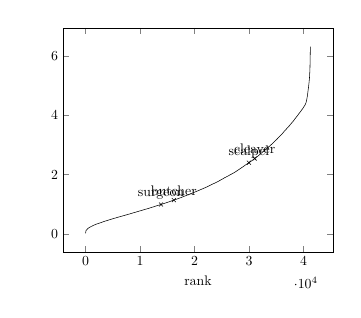
\begin{tikzpicture} [scale=0.5]
	\begin{axis} [xlabel=rank,ylabel=PMI,y label style={color=white}]
	\addplot [mark=none] coordinates {
(0,0.01004) (82,0.10112) (164,0.12417) (246,0.14062) (328,0.15755) (410,0.17296) (492,0.18456) (574,0.19468) (656,0.20589) (738,0.21453) (820,0.22473) (902,0.23274) (984,0.2401) (1066,0.24851) (1148,0.25546) (1230,0.26299) (1312,0.27054) (1394,0.27863) (1476,0.28481) (1558,0.2915) (1640,0.29752) (1722,0.30343) (1804,0.30956) (1886,0.31675) (1968,0.32333) (2050,0.32831) (2132,0.33313) (2214,0.3384) (2296,0.34394) (2378,0.34814) (2460,0.3538) (2542,0.35913) (2624,0.36444) (2706,0.36953) (2788,0.37487) (2870,0.37967) (2952,0.38513) (3034,0.38953) (3116,0.39547) (3198,0.40102) (3280,0.40585) (3362,0.41063) (3444,0.41565) (3526,0.42068) (3608,0.42616) (3690,0.4312) (3772,0.43623) (3854,0.44049) (3936,0.44462) (4018,0.44953) (4100,0.45438) (4182,0.45911) (4264,0.46431) (4346,0.46947) (4428,0.47387) (4510,0.47886) (4592,0.48422) (4674,0.48876) (4756,0.4925) (4838,0.49659) (4920,0.50107) (5002,0.50641) (5084,0.51135) (5166,0.51547) (5248,0.51932) (5330,0.52409) (5412,0.52829) (5494,0.53188) (5576,0.53712) (5658,0.5434) (5740,0.54751) (5822,0.55141) (5904,0.55585) (5986,0.56004) (6068,0.56406) (6150,0.56827) (6232,0.57183) (6314,0.57573) (6396,0.58003) (6478,0.58505) (6560,0.58909) (6642,0.5938) (6724,0.59793) (6806,0.60156) (6888,0.60534) (6970,0.61003) (7052,0.61445) (7134,0.61962) (7216,0.62455) (7298,0.62823) (7380,0.63238) (7462,0.63603) (7544,0.64026) (7626,0.64493) (7708,0.64952) (7790,0.65361) (7872,0.65815) (7954,0.66269) (8036,0.66683) (8118,0.67159) (8200,0.67607) (8282,0.67947) (8364,0.68488) (8446,0.68908) (8528,0.69304) (8610,0.69802) (8692,0.70339) (8774,0.70777) (8856,0.71124) (8938,0.71568) (9020,0.7198) (9102,0.7239) (9184,0.72878) (9266,0.73343) (9348,0.73723) (9430,0.74189) (9512,0.74635) (9594,0.75065) (9676,0.7557) (9758,0.75996) (9840,0.76391) (9922,0.76901) (10004,0.77353) (10086,0.77779) (10168,0.78219) (10250,0.78652) (10332,0.79145) (10414,0.79531) (10496,0.80012) (10578,0.80532) (10660,0.80945) (10742,0.81342) (10824,0.81732) (10906,0.82221) (10988,0.82745) (11070,0.83131) (11152,0.83563) (11234,0.83974) (11316,0.84422) (11398,0.84898) (11480,0.85286) (11562,0.85717) (11644,0.86237) (11726,0.86768) (11808,0.87183) (11890,0.8768) (11972,0.88124) (12054,0.88766) (12136,0.89174) (12218,0.89593) (12300,0.9004) (12382,0.90499) (12464,0.91022) (12546,0.91524) (12628,0.92063) (12710,0.92589) (12792,0.9302) (12874,0.93491) (12956,0.93958) (13038,0.94382) (13120,0.94897) (13202,0.95368) (13284,0.95825) (13366,0.96291) (13448,0.96773) (13530,0.97199) (13612,0.9763) (13694,0.98069) (13776,0.98459) (13858,0.98966) (13940,0.99399) (14022,0.99876) (14104,1.00333) (14186,1.00931) (14268,1.01341) (14350,1.01921) (14432,1.02376) (14514,1.02881) (14596,1.0337) (14678,1.03876) (14760,1.04444) (14842,1.04948) (14924,1.05469) (15006,1.05989) (15088,1.06474) (15170,1.06996) (15252,1.07588) (15334,1.08069) (15416,1.08643) (15498,1.09186) (15580,1.09734) (15662,1.10242) (15744,1.10785) (15826,1.11413) (15908,1.11883) (15990,1.1244) (16072,1.12913) (16154,1.13446) (16236,1.13927) (16318,1.14435) (16400,1.15018) (16482,1.15522) (16564,1.16049) (16646,1.16489) (16728,1.1701) (16810,1.17582) (16892,1.18192) (16974,1.18815) (17056,1.19322) (17138,1.19823) (17220,1.20358) (17302,1.20987) (17384,1.21516) (17466,1.21968) (17548,1.22499) (17630,1.23088) (17712,1.23803) (17794,1.24268) (17876,1.24986) (17958,1.25649) (18040,1.2622) (18122,1.26725) (18204,1.27383) (18286,1.28019) (18368,1.28526) (18450,1.29071) (18532,1.29788) (18614,1.30401) (18696,1.30931) (18778,1.31475) (18860,1.32057) (18942,1.32722) (19024,1.33404) (19106,1.33982) (19188,1.34682) (19270,1.3532) (19352,1.35828) (19434,1.36399) (19516,1.36963) (19598,1.37588) (19680,1.38155) (19762,1.38811) (19844,1.3934) (19926,1.39918) (20008,1.40595) (20090,1.41118) (20172,1.41886) (20254,1.42561) (20336,1.4322) (20418,1.43866) (20500,1.44371) (20582,1.44929) (20664,1.45499) (20746,1.46161) (20828,1.46834) (20910,1.47572) (20992,1.48208) (21074,1.48938) (21156,1.49567) (21238,1.502) (21320,1.50777) (21402,1.51482) (21484,1.52101) (21566,1.52692) (21648,1.53378) (21730,1.5405) (21812,1.54756) (21894,1.55427) (21976,1.56093) (22058,1.56736) (22140,1.57399) (22222,1.58047) (22304,1.58707) (22386,1.59404) (22468,1.60202) (22550,1.61023) (22632,1.61838) (22714,1.62572) (22796,1.63352) (22878,1.64017) (22960,1.6482) (23042,1.65694) (23124,1.66455) (23206,1.66957) (23288,1.67764) (23370,1.68445) (23452,1.69159) (23534,1.69743) (23616,1.7047) (23698,1.71182) (23780,1.71945) (23862,1.72803) (23944,1.73609) (24026,1.74283) (24108,1.74953) (24190,1.75746) (24272,1.76496) (24354,1.77295) (24436,1.7803) (24518,1.78909) (24600,1.79816) (24682,1.80732) (24764,1.81569) (24846,1.82402) (24928,1.83185) (25010,1.83983) (25092,1.84653) (25174,1.85539) (25256,1.86431) (25338,1.87298) (25420,1.88129) (25502,1.89292) (25584,1.90107) (25666,1.90717) (25748,1.91474) (25830,1.92326) (25912,1.93098) (25994,1.93822) (26076,1.94552) (26158,1.95458) (26240,1.96421) (26322,1.97138) (26404,1.98058) (26486,1.98953) (26568,1.99806) (26650,2.0048) (26732,2.01379) (26814,2.02163) (26896,2.03003) (26978,2.0378) (27060,2.04688) (27142,2.05528) (27224,2.06416) (27306,2.0726) (27388,2.08179) (27470,2.09186) (27552,2.1006) (27634,2.11046) (27716,2.11894) (27798,2.12917) (27880,2.14078) (27962,2.15169) (28044,2.16215) (28126,2.17069) (28208,2.18003) (28290,2.1901) (28372,2.20237) (28454,2.21281) (28536,2.22127) (28618,2.23267) (28700,2.24393) (28782,2.25311) (28864,2.26285) (28946,2.27433) (29028,2.28413) (29110,2.29509) (29192,2.30673) (29274,2.31722) (29356,2.3273) (29438,2.3381) (29520,2.34938) (29602,2.35963) (29684,2.36963) (29766,2.37996) (29848,2.38884) (29930,2.39786) (30012,2.40662) (30094,2.41785) (30176,2.42997) (30258,2.43904) (30340,2.44846) (30422,2.45941) (30504,2.47207) (30586,2.48308) (30668,2.49381) (30750,2.50379) (30832,2.51552) (30914,2.5269) (30996,2.53916) (31078,2.55115) (31160,2.56154) (31242,2.57291) (31324,2.58307) (31406,2.59604) (31488,2.60689) (31570,2.61998) (31652,2.63238) (31734,2.64579) (31816,2.65861) (31898,2.67144) (31980,2.68472) (32062,2.69803) (32144,2.712) (32226,2.72464) (32308,2.73657) (32390,2.74777) (32472,2.75953) (32554,2.77461) (32636,2.78639) (32718,2.79994) (32800,2.81118) (32882,2.82421) (32964,2.83656) (33046,2.84961) (33128,2.8645) (33210,2.87854) (33292,2.89033) (33374,2.90405) (33456,2.91733) (33538,2.92832) (33620,2.94034) (33702,2.95501) (33784,2.96828) (33866,2.98301) (33948,2.99515) (34030,3.00776) (34112,3.02234) (34194,3.03712) (34276,3.05141) (34358,3.06588) (34440,3.07913) (34522,3.09254) (34604,3.10971) (34686,3.12494) (34768,3.1389) (34850,3.15573) (34932,3.16772) (35014,3.17953) (35096,3.19689) (35178,3.20979) (35260,3.22681) (35342,3.24166) (35424,3.25793) (35506,3.27277) (35588,3.28864) (35670,3.30331) (35752,3.32018) (35834,3.33539) (35916,3.34992) (35998,3.36567) (36080,3.38042) (36162,3.39874) (36244,3.42298) (36326,3.43814) (36408,3.45543) (36490,3.472) (36572,3.48727) (36654,3.50482) (36736,3.5231) (36818,3.53751) (36900,3.55525) (36982,3.57058) (37064,3.58827) (37146,3.60348) (37228,3.6211) (37310,3.63785) (37392,3.6537) (37474,3.67321) (37556,3.69422) (37638,3.70843) (37720,3.72642) (37802,3.74467) (37884,3.76195) (37966,3.782) (38048,3.79854) (38130,3.81529) (38212,3.83622) (38294,3.85617) (38376,3.8778) (38458,3.89704) (38540,3.91657) (38622,3.93641) (38704,3.95512) (38786,3.97558) (38868,3.99189) (38950,4.01043) (39032,4.03438) (39114,4.05616) (39196,4.07354) (39278,4.09439) (39360,4.11559) (39442,4.13547) (39524,4.15566) (39606,4.17789) (39688,4.19701) (39770,4.21642) (39852,4.23612) (39934,4.25803) (40016,4.28428) (40098,4.31039) (40180,4.33158) (40262,4.35509) (40344,4.38619) (40426,4.42515) (40508,4.47456) (40590,4.55117) (40672,4.63453) (40754,4.74044) (40836,4.86945) (40918,4.977) (41000,5.1181) (41082,5.27117) (41164,5.55781) (41246,6.33026)
	};
	\addplot [mark=x,only marks] coordinates {
		(13845,0.98899)(16190,1.13695)(29968,2.40174)(31024,2.54414)
	};
	\node [anchor=south] at (axis cs: 13845,0.98899) {surgeon};
	\node [anchor=south] at (axis cs: 16190,1.13695) {butcher};
	\node [anchor=south] at (axis cs: 29968,2.40174) {scalpel};
	\node [anchor=south] at (axis cs: 31024,2.54414) {cleaver};
	\end{axis}
\end{tikzpicture}
\caption{dimension: \emph{hands}}
\end{subfigure}
\centering
\begin{subfigure} [t] {0.3 \textwidth}
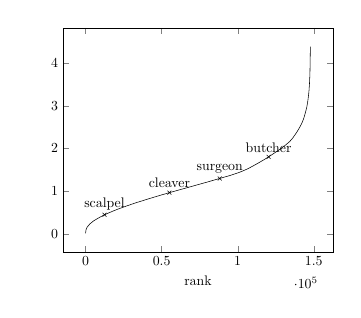
\begin{tikzpicture} [scale=0.5]
	\begin{axis} [xlabel=rank,ylabel=PMI,y label style={color=white}]
	\addplot [mark=none] coordinates {
		(0,0.00873) (295,0.08756) (590,0.12013) (885,0.14286) (1180,0.1607) (1475,0.17372) (1770,0.18662) (2065,0.20012) (2360,0.21206) (2655,0.22349) (2950,0.23441) (3245,0.24433) (3540,0.25194) (3835,0.26042) (4130,0.26934) (4425,0.27875) (4720,0.28699) (5015,0.29465) (5310,0.30183) (5605,0.30913) (5900,0.31561) (6195,0.32201) (6490,0.32861) (6785,0.33471) (7080,0.3407) (7375,0.3472) (7670,0.35305) (7965,0.35943) (8260,0.36555) (8555,0.37194) (8850,0.37792) (9145,0.38409) (9440,0.38982) (9735,0.39532) (10030,0.40097) (10325,0.4068) (10620,0.41244) (10915,0.4175) (11210,0.42332) (11505,0.4289) (11800,0.43381) (12095,0.43959) (12390,0.44398) (12685,0.44896) (12980,0.45406) (13275,0.45911) (13570,0.4639) (13865,0.46904) (14160,0.47337) (14455,0.47822) (14750,0.48215) (15045,0.48676) (15340,0.49105) (15635,0.4958) (15930,0.50037) (16225,0.50464) (16520,0.50927) (16815,0.51314) (17110,0.5178) (17405,0.5226) (17700,0.52745) (17995,0.53188) (18290,0.53667) (18585,0.54042) (18880,0.54459) (19175,0.54871) (19470,0.55311) (19765,0.55732) (20060,0.56142) (20355,0.56567) (20650,0.5698) (20945,0.57383) (21240,0.57791) (21535,0.58164) (21830,0.58552) (22125,0.58925) (22420,0.59313) (22715,0.59699) (23010,0.60082) (23305,0.60506) (23600,0.60903) (23895,0.61294) (24190,0.61639) (24485,0.62025) (24780,0.62395) (25075,0.62797) (25370,0.6315) (25665,0.63521) (25960,0.63898) (26255,0.64253) (26550,0.64675) (26845,0.65017) (27140,0.65398) (27435,0.65793) (27730,0.66142) (28025,0.66484) (28320,0.66857) (28615,0.67248) (28910,0.67612) (29205,0.67968) (29500,0.68328) (29795,0.68728) (30090,0.69088) (30385,0.69415) (30680,0.69775) (30975,0.70109) (31270,0.70435) (31565,0.70817) (31860,0.71161) (32155,0.71545) (32450,0.71891) (32745,0.72262) (33040,0.72637) (33335,0.72966) (33630,0.7331) (33925,0.73667) (34220,0.73973) (34515,0.74279) (34810,0.7459) (35105,0.74919) (35400,0.75252) (35695,0.75606) (35990,0.75912) (36285,0.76252) (36580,0.76565) (36875,0.76909) (37170,0.7723) (37465,0.77577) (37760,0.77899) (38055,0.78258) (38350,0.78613) (38645,0.78925) (38940,0.79236) (39235,0.79558) (39530,0.79895) (39825,0.80261) (40120,0.80618) (40415,0.8093) (40710,0.81259) (41005,0.81587) (41300,0.8189) (41595,0.822) (41890,0.82529) (42185,0.82836) (42480,0.831) (42775,0.8342) (43070,0.83738) (43365,0.84046) (43660,0.84368) (43955,0.84705) (44250,0.8503) (44545,0.8539) (44840,0.8571) (45135,0.86037) (45430,0.8634) (45725,0.86668) (46020,0.86967) (46315,0.87284) (46610,0.87596) (46905,0.87934) (47200,0.88226) (47495,0.88532) (47790,0.88815) (48085,0.89148) (48380,0.89464) (48675,0.89792) (48970,0.90121) (49265,0.90408) (49560,0.90712) (49855,0.9105) (50150,0.91355) (50445,0.91662) (50740,0.9196) (51035,0.92264) (51330,0.92587) (51625,0.92858) (51920,0.9317) (52215,0.93476) (52510,0.93752) (52805,0.94067) (53100,0.94403) (53395,0.94684) (53690,0.94973) (53985,0.9531) (54280,0.95608) (54575,0.95903) (54870,0.96235) (55165,0.96528) (55460,0.96823) (55755,0.9709) (56050,0.97389) (56345,0.97714) (56640,0.98012) (56935,0.98296) (57230,0.98571) (57525,0.98879) (57820,0.99174) (58115,0.99439) (58410,0.99753) (58705,1.00047) (59000,1.00323) (59295,1.00594) (59590,1.00932) (59885,1.01223) (60180,1.01548) (60475,1.01823) (60770,1.02118) (61065,1.02405) (61360,1.02711) (61655,1.03007) (61950,1.03277) (62245,1.03554) (62540,1.03864) (62835,1.04148) (63130,1.04441) (63425,1.04769) (63720,1.05068) (64015,1.05349) (64310,1.05632) (64605,1.05917) (64900,1.06239) (65195,1.06491) (65490,1.06798) (65785,1.071) (66080,1.07403) (66375,1.07658) (66670,1.07991) (66965,1.08284) (67260,1.08551) (67555,1.08852) (67850,1.09125) (68145,1.09441) (68440,1.09761) (68735,1.10049) (69030,1.10307) (69325,1.10642) (69620,1.10932) (69915,1.11248) (70210,1.11485) (70505,1.11804) (70800,1.12124) (71095,1.12447) (71390,1.12701) (71685,1.13009) (71980,1.13278) (72275,1.13605) (72570,1.13922) (72865,1.14204) (73160,1.14507) (73455,1.1477) (73750,1.15088) (74045,1.15353) (74340,1.15627) (74635,1.15954) (74930,1.16242) (75225,1.16531) (75520,1.16823) (75815,1.17134) (76110,1.17439) (76405,1.17706) (76700,1.18063) (76995,1.18332) (77290,1.18603) (77585,1.18921) (77880,1.19209) (78175,1.19502) (78470,1.19791) (78765,1.20069) (79060,1.20348) (79355,1.20629) (79650,1.20911) (79945,1.21241) (80240,1.21555) (80535,1.21861) (80830,1.22149) (81125,1.22487) (81420,1.22827) (81715,1.2312) (82010,1.23414) (82305,1.2371) (82600,1.24007) (82895,1.24306) (83190,1.24607) (83485,1.24909) (83780,1.25212) (84075,1.25535) (84370,1.25824) (84665,1.26133) (84960,1.26442) (85255,1.26754) (85550,1.27015) (85845,1.27382) (86140,1.27646) (86435,1.27964) (86730,1.28301) (87025,1.28595) (87320,1.28874) (87615,1.29198) (87910,1.29524) (88205,1.29761) (88500,1.30072) (88795,1.3032) (89090,1.30647) (89385,1.30959) (89680,1.31294) (89975,1.31632) (90270,1.31929) (90565,1.32248) (90860,1.32542) (91155,1.32867) (91450,1.3314) (91745,1.33452) (92040,1.33719) (92335,1.34049) (92630,1.34284) (92925,1.34614) (93220,1.34875) (93515,1.35203) (93810,1.35513) (94105,1.35834) (94400,1.36124) (94695,1.3644) (94990,1.36758) (95285,1.37061) (95580,1.37423) (95875,1.37795) (96170,1.38107) (96465,1.38484) (96760,1.38799) (97055,1.39179) (97350,1.3951) (97645,1.39904) (97940,1.40205) (98235,1.40594) (98530,1.40985) (98825,1.41309) (99120,1.41642) (99415,1.42032) (99710,1.4238) (100005,1.42707) (100300,1.43096) (100595,1.43467) (100890,1.4381) (101185,1.44215) (101480,1.44614) (101775,1.4503) (102070,1.45448) (102365,1.45869) (102660,1.46256) (102955,1.46711) (103250,1.47148) (103545,1.4758) (103840,1.48063) (104135,1.48506) (104430,1.4899) (104725,1.49483) (105020,1.4993) (105315,1.50405) (105610,1.50883) (105905,1.51364) (106200,1.51823) (106495,1.52355) (106790,1.52829) (107085,1.5334) (107380,1.53849) (107675,1.54404) (107970,1.54991) (108265,1.55528) (108560,1.56097) (108855,1.56671) (109150,1.57221) (109445,1.57817) (109740,1.58419) (110035,1.58962) (110330,1.59523) (110625,1.60124) (110920,1.60644) (111215,1.6124) (111510,1.61807) (111805,1.62349) (112100,1.62939) (112395,1.63614) (112690,1.64192) (112985,1.64777) (113280,1.65342) (113575,1.65958) (113870,1.6656) (114165,1.6715) (114460,1.67753) (114755,1.68362) (115050,1.69056) (115345,1.69642) (115640,1.70314) (115935,1.70894) (116230,1.71511) (116525,1.72116) (116820,1.72726) (117115,1.7334) (117410,1.7396) (117705,1.7455) (118000,1.75179) (118295,1.75814) (118590,1.76493) (118885,1.77188) (119180,1.77858) (119475,1.78441) (119770,1.79103) (120065,1.7977) (120360,1.8048) (120655,1.81196) (120950,1.81804) (121245,1.82571) (121540,1.83226) (121835,1.83877) (122130,1.84628) (122425,1.85314) (122720,1.85995) (123015,1.86691) (123310,1.87338) (123605,1.8807) (123900,1.88815) (124195,1.89467) (124490,1.90165) (124785,1.90879) (125080,1.91606) (125375,1.92384) (125670,1.93038) (125965,1.93784) (126260,1.94493) (126555,1.95164) (126850,1.95975) (127145,1.96748) (127440,1.97439) (127735,1.9813) (128030,1.98876) (128325,1.99629) (128620,2.00293) (128915,2.0101) (129210,2.0185) (129505,2.02609) (129800,2.0342) (130095,2.04288) (130390,2.05098) (130685,2.05863) (130980,2.06739) (131275,2.07588) (131570,2.08472) (131865,2.09207) (132160,2.10107) (132455,2.11016) (132750,2.11881) (133045,2.12863) (133340,2.13745) (133635,2.14679) (133930,2.15536) (134225,2.16597) (134520,2.17709) (134815,2.1879) (135110,2.20013) (135405,2.21217) (135700,2.22397) (135995,2.23776) (136290,2.25101) (136585,2.26502) (136880,2.28041) (137175,2.29604) (137470,2.3102) (137765,2.32542) (138060,2.3402) (138355,2.35664) (138650,2.37329) (138945,2.38835) (139240,2.40539) (139535,2.42262) (139830,2.43996) (140125,2.45796) (140420,2.47517) (140715,2.49428) (141010,2.51376) (141305,2.53363) (141600,2.55316) (141895,2.57224) (142190,2.59489) (142485,2.6199) (142780,2.6466) (143075,2.67209) (143370,2.70154) (143665,2.73407) (143960,2.77034) (144255,2.80907) (144550,2.84553) (144845,2.88325) (145140,2.92826) (145435,2.97315) (145730,3.03039) (146025,3.09462) (146320,3.17092) (146615,3.25689) (146910,3.36659) (147205,3.52351) (147500,3.75669) (147795,4.38804)
	};
	\addplot [mark=x,only marks] coordinates {
		(12466,0.44529)(55096,0.9647)(88206,1.29763)(120293,1.80307)
	};
	\node [anchor=south] at (axis cs: 12466,0.44529) {scalpel};
	\node [anchor=south] at (axis cs: 55096,0.9647) {cleaver};
	\node [anchor=south] at (axis cs: 88206,1.29763) {surgeon};
	\node [anchor=south] at (axis cs: 120293,1.80307) {butcher};
	\end{axis}
\end{tikzpicture}
\caption{dimension: \emph{known}}
\end{subfigure}
\caption[The Arithmetic of Analogy]{Histograms of the top three co-occurrence dimensions satisfying the expected arithmetic of analogy.}
\label{FIG:histograms}
\end{figure}

\begin{figure}
\centering
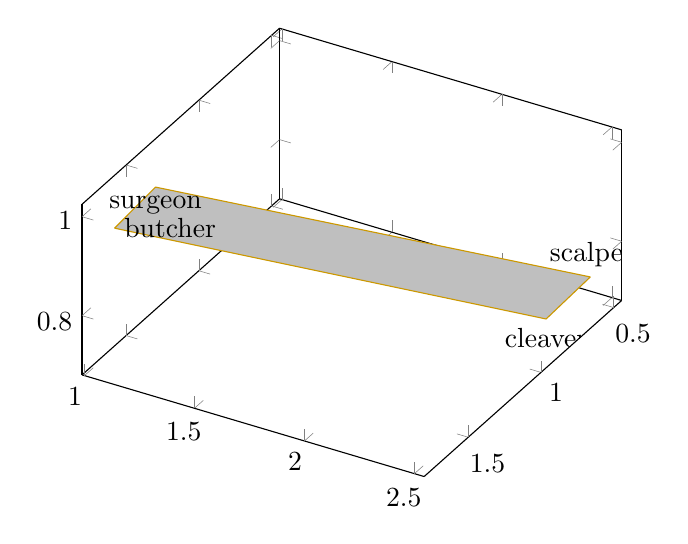
\begin{tikzpicture}
%\begin{axis}[view={120}{10},xmin=0,xmax=4.5,ymin=0,ymax=4.5,zmin=0,zmax=4.5,xlabel=gray,ylabel=relate, zlabel=tone,colormap/blackwhite]
\begin{axis}[view={120}{50}]
%\addplot3 [color=black,->,ultra thick] coordinates {(0,0,0) (4,4,4)};
\addplot3[patch,patch type=rectangle,color=lightgray,fill opacity=1] coordinates {
 	(0.44529,2.40174,0.70908) (0.9647,2.54414,0.77903) (1.80307,1.13695,0.99632) (1.2979763,0.98899,0.92747)
};
\node [anchor=south] at (axis cs: 0.44529,2.40174,0.70908) {scalpel};
\node [anchor=north] at (axis cs: 0.9647,2.54414,0.77903) {cleaver};
\node [anchor=north] at (axis cs: 1.2979763,0.98899,0.92747) {surgeon};
\node [anchor=west] at (axis cs: 1.80307,1.13695,0.99632) {butcher};
%\addplot3 [color=black,->,ultra thick] coordinates {(2.2,2.2,2.2) (4,4,4)};
\end{axis}
\end{tikzpicture}
\caption{An Analogy in Space. When the analogue values of the three dimensions described in Figure~\ref{FIG:histograms} are plotted, the analogy itself emerges as a parallelogram situated obliquely in the centre of the positive region of the space.}
\label{FIG:subspace}
\end{figure}

\begin{figure}
\centering
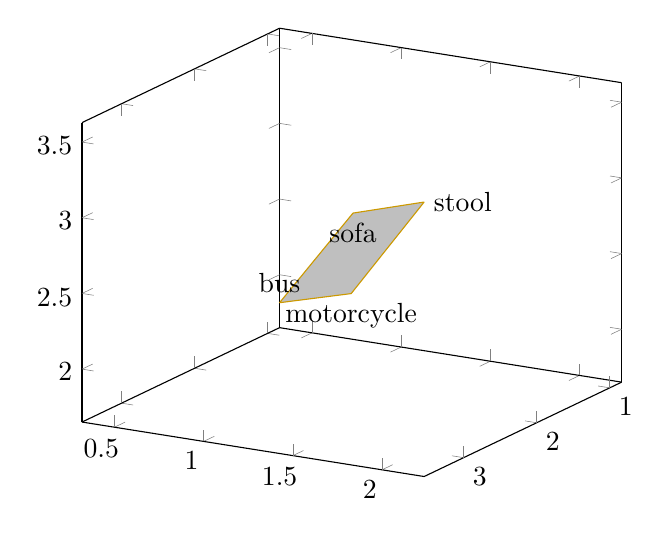
\begin{tikzpicture}
%\begin{axis}[view={120}{10},xmin=0,xmax=4.5,ymin=0,ymax=4.5,zmin=0,zmax=4.5,xlabel=gray,ylabel=relate, zlabel=tone,colormap/blackwhite]
\begin{axis}[view={120}{20}]
%\addplot3 [color=black,->,ultra thick] coordinates {(0,0,0) (4,4,4)};
\addplot3[patch,patch type=rectangle,color=lightgray,fill opacity=1] coordinates {
 	(0.83647,0.3181,1.81529) (1.05531,0.80923,2.01808) (3.5408,2.23614,3.46375) (3.32574,1.74923,3.24988)
};
\node [anchor=south] at (axis cs: 0.83647,0.3181,1.81529) {bus};
\node [anchor=north] at (axis cs: 1.05531,0.80923,2.01808) {motorcycle};
\node [anchor=north] at (axis cs: 3.32574,1.74923,3.24988) {sofa};
\node [anchor=west] at (axis cs: 3.5408,2.23614,3.46375) {stool};
%\addplot3 [color=black,->,ultra thick] coordinates {(2.2,2.2,2.2) (4,4,4)};
\end{axis}
\end{tikzpicture}
\caption{An Analogy in Space. When the analogue values of the three dimensions described in Figure~\ref{FIG:histograms} are plotted, the analogy itself emerges as a parallelogram situated obliquely in the centre of the positive region of the space.}
\label{FIG:subspace}
\end{figure}

\subsection{Projecting Probability in Space}

\subsection{Finding Contexts for Analogies}
\begin{table}
\centering
\begin{tabular}{clrrrrrr}
\hline
\multicolumn{2}{l}{\emph{dimensions}} & 5 & 10 & 20 & 50 & 100 & 200 \\
\hline
\parbox[t]{2mm}{\multirow{4}{*}{\rotatebox[origin=c]{90}{ 2x2}}} & \textsc{joint} & 0.911 & 0.972 & 0.989 & 0.986 & 0.970 & 0.916 \\
& \textsc{indy} & 0.000 & 0.000 & 0.001 & 0.090 & 0.356 & 0.677 \\
& \textsc{zipped} & 0.921 & 0.975 & 0.991 & 0.987 & 0.970 & 0.919 \\
\hline
\parbox[t]{2mm}{\multirow{4}{*}{\rotatebox[origin=c]{90}{\textsc{ 5x5}}}} & \textsc{joint} & 0.941 & 0.987 & 0.996 & 0.997 & 0.957 \\
& \textsc{indy} & 0.000 & 0.000 & 0.012 & 0.098 & 0.202 & 0.610 \\
& \textsc{zipped} & 0.934 & 0.987 & 0.999 & 0.998 & 0.997 & 0.968 \\
\hline
\end{tabular}
\caption[Finding Spaces for Known Analogies]{Accuracy rates for solving analogies when choosing subsets of optimal dimensions from 400 dimensional subspaces picked taking the first three elements of each analogy as input.}
\end{table}

\begin{table}
\centering
\begin{tabular}{clrrrrrr}
\hline
\multicolumn{2}{l}{\emph{dimensions}} & 5 & 10 & 20 & 50 & 100 & 200 \\
\hline
\parbox[t]{2mm}{\multirow{4}{*}{\rotatebox[origin=c]{90}{2x2}}} & \textsc{joint} & 0.654 & 0.814 & 0.896 & 0.930 & 0.881 & 0.466 \\
& \textsc{indy} & 0.000 & 0.000 & 0.000 & 0.072 & 0.356 & 0.636 \\
& \textsc{zipped} & 0.616 & 0.806 & 0.892 & 0.929 & 0.887 & 0.489 \\
\hline
\parbox[t]{2mm}{\multirow{4}{*}{\rotatebox[origin=c]{90}{\textsc{5x5}}}} & \textsc{joint} & 0.657 & 0.828 & 0.901 & 0.921 & 0.835 & 0.402 \\
& \textsc{indy} & 0.000 & 0.000 & 0.003 & 0.074 & 0.225 & 0.569 \\
& \textsc{zipped} & 0.589 & 0.790 & 0.888 & 0.915 & 0.876 & 0.418 \\
\hline
\end{tabular}
\caption[Finding Spaces for Fake Analogies]{Accuracy rates for solving randomly completed analogies when choosing subsets of optimal dimensions from 400 dimensional subspaces picked taking the first three elements of each analogy as input.}
\end{table}

\begin{figure}
  \begin{tikzpicture}
    \begin{axis}[scatter/classes={x={mark=x,draw=black},o={mark=o,draw=black}}]
      \addplot[scatter,only marks,scatter src=explicit symbolic]
      table[meta=label] {
      x y label
      1 1 x
      2 0 o
      };
    \end{axis}
  \end{tikzpicture}
\end{figure}

\section{A Note on the Data}
It must be mentioned that the data that has been analysed in this chapter is of a very specific character.  The analogies put together by the team at Google are populated by a high percentage of proper names, in particular place names and also currencies, demonyms, and the like.  This belies a particular view of language and indeed cognition which is at odds with the premise motivating the model described in this thesis, as outlined at the beginning of Chapter~\ref{chap:theory}.  Proper names are, as \cite{Russell} has pointed out, particular kinds of words with peculiar denotational properties in that they refer to specific and unique entities or correspondingly specific classes of entities.  This is not to say that they do not admit ambiguity -- \emph{Paris} is the name of, among other things, a classical character, and \emph{Berlin} the name of a 1980s new wave band -- but there tends to be a certain clarity of intent when these types of words are used.  These types of analogies are exemplary of cases where language coalesces into a relatively stable conceptual representation, and, notwithstanding cases of polysemy, it's arguably not particularly surprising that these relationships emerge as commensurable directions in a likewise stable representational space.

Furthermore, it is telling that the designers of the dataset have chosen to refer to the variety of analogy typified by \emph{slow:slowly::fast:quickly} as \emph{syntactic}.  With reference to \cite{Saussure} and more lately in the distributional semantic paradigm \cite{Sahlgren}, I would rather call this type of analogy \emph{syntagmatic}, in that 
